% !BIB TS-program = biber
\documentclass[11pt]{article}

\usepackage{graphicx}
\usepackage{hyperref}
\usepackage{amsmath}
\usepackage[style=authoryear,backend=biber,mincitenames=1,maxcitenames=2, uniquelist=false]{biblatex}
\bibliography{fossilDating.bib}


\newcommand{\Mstrict}{{M1}}
\newcommand{\Mrelaxed}{{M8}}

\begin{document}

\title{Bayesian phylogenetic estimation of fossil ages reveals remarkable consistency of rocks and clocks}
\author{Alexei Drummond, Tanja Stadler}
\date{\today{}}
\maketitle

% 250 words
\abstract{
Recent advances have allowed for both morphological fossil evidence and molecular sequence data to be integrated into a single combined inference of divergence dates under the rule of Bayesian probability. 
In particular the fossilized birth-death tree prior and the Lewis-MK model of evolution of discrete morphological change allow for the estimation of both divergence times and the phylogenetic relationships between fossil and extant taxa. 
We exploit this statistical framework to investigate the internal consistency of these models by estimating the phylogenetic age of each fossil in turn, within a rich and well-characterized data set of fossil and extant penguins.
We find that we can accurately estimate the age of individual penguin fossils based only on phylogenetic evidence. 
In fact in the data set we analyze the {\em phylogenetic age} of a fossil species is on average only 2 My from the midpoint age of the geological strata from which the fossil species was excavated. 
The high level of internal consistency found in our analyses provides strong evidence that the Bayesian statistical model employed is a good fit for both the palaeontological and molecular data, and provides striking evidence from a real data set that the framework used can accurately model the evolution of discrete morphological traits coded from fossil and extant taxa. 
We anticipate that this approach will have diverse applications including estimating dates for fossils that are temporally unconstrained, testing the ``morphological clock'', and as part of evaluating model assumptions when controversial phylogenetic hypotheses are obtained based on morphological data.
}

\section*{Introduction}

% Papers
% http://www.ncbi.nlm.nih.gov/pmc/articles/PMC4033271/ Beyond fossil calibrations: realities of molecular clock practices in evolutionary biology
% http://journals.plos.org/plosone/article?id=10.1371/journal.pone.0066245 A Simple Method for Estimating Informative Node Age Priors for the Fossil Calibration of Molecular Divergence Time Analyses
% http://www.ncbi.nlm.nih.gov/pmc/articles/PMC3108556/  Bayesian Phylogenetic Method to Estimate Unknown Sequence Ages
% http://www.pnas.org/content/112/16/4897 Canids

Although there has been much controversy surrounding apparent discrepancies between palaeontological data and molecular phylogenetic inferences it is clear that fossil and molecular data both produce broadly concordant views of evolutionary history\footnote{For example see \url{http://www.actionbioscience.org/evolution/benton.html}}. 
Indeed one of the first examples of endeavouring to apply a macroevolutionary phylogenetic model to perform inference directly on fossil occurrence data in fact demonstrated concordance between inferences from  molecular data and paleontological data in primates \autocite{tavare2002using}. 
% AJD: The following two sentences are inflammatory to palaeontologists
%Nevertheless there have been only few attempts to apply phylogenetic reasoning to palaeontological questions. 
%Models of molecular evolution have been refined over many decades \autocite{Felsenstein2004,Yang:2006yu}. 
The continual improvement of models and methods for statistical phylogenetic inference of molecular sequence data is well documented \autocite[e.g.][]{Felsenstein2004,Yang:2006yu}. 
However, it may be less widely appreciated by molecular evolutionary biologists that phylogenetic reasoning has also been heavily applied to palaeontological questions including to questions of biogeography, character evolution, and the completeness of the fossil record.
In particular probabilistic model based approaches to biogeography, ancestral state reconstruction, and rates of morphological character change have been common in recent years. But the application of phylogenetic approaches to palaeontological questions extends back for decades. Nevertheless there has been a call by some palaeontologists for 
%The earlier literature is awash with research papers that include fossils in phylogenies, utilize a phylogenetic bracket to constrain inferences of soft tissue or physiology, or use trees to reconstruct biogeography.

Traditionally the practice has been to use a fossil as a ``node calibration'' by associated its geologically-derived age to a particular divergence in a molecular phylogeny. The age can be derived by radiometric aging of strata above and/or below the strata, or by biostratigraphy wish employs This node calibration then confers age estimates to the remaining divergences on a phylogenetic tree by the assumption of a strict or relaxed molecular clock \autocite{Thorne1998,thorne2005,yang2006,Drummond2006}. 
Here we instead focus on what phylogenetic inference techniques can tell us about the ``phylogenetic age'' of a fossil, based solely on its morphological characteristics.
\subsection*{Phylogenetic tip-dating}

The phylogenetic estimation of the age of a taxon based on its molecular sequence has been previously described \autocite{drummond2002computational,shapiro2011bayesian} and applied to both ancient subfossil remains and rapidly evolving viral taxa. For example, this technique has been successfully employed to estimate the age of human subfossil remains based on an ancient mitochondrial genome sequence \autocite{meyer2014mitochondrial}. The same technique has also been used to estimate the age of viral samples based on molecular sequence data \autocite[e.g.][]{gray2013evolutionary}.

We extend this work into the realm of morphological evolution by presenting a statistical model of evolution that generates an expectation on the distribution of fossils and their morphological characters. This model has been previously presented in the context of divergence time dating \autocite{gavr2014,gavryushkina2015bayesian}. It is distinct from alternative divergence time dating approaches in that is provides an explicit treatment of the temporal information contained in fossil remains, whether or not related molecular sequence data is available. This leads to an estimate of the age of the most recent common ancestor of a group of fossils. We exploit this framework to attempt the estimation of the phylogenetic age of individual fossils based solely on morphological data and their phylogenetic affinities to related fossils of known age. The method is applied to a rich and well-characterized morphological data set of extant penguins and their fossil ancestors \autocite{ksepka2010,ksepka2012}.

\section*{Methods}

\textcite{gavryushkina2015bayesian} described a ``total-evidence'' approach to the phylogenetic estimation of time-trees that employed both fossil and molecular sequence data as equal partners under the rule of probability. We extend their work further by investigating the consistency between the estimated phylogenetic age of a fossil and the corresponding palaeontological age range based on radiometrically-dated geological strata. The model of time-tree phylogeny employed is the so-called fossilized birth-death process \autocite{Heath2014}, which forms a prior probability distribution on the space of sampled-ancestor trees \autocite{Gavr2013}.

A previous study described how a set of fossils with discrete morphological characters could be used to estimate a time-tree or chrono-phylogeny. Here we additionally allow for one or more of the fossils to have broad uninformative priors on their age. This allows for the age of some of the fossils to be estimated solely based on their morphological characters and the phylogenetic affinities of their morphology to other fossils with known ages in the time-tree. We refer to this estimate of a fossil's age as its {\em phylogenetic age}. In estimating each of the fossils' phylogenetic ages in turn, three questions can be answered: (i) How much information about an individual fossil's age is available from phylogenetic analysis of morphological data alone, (ii) What is the level of phylogenetic evidence in support of the palaeontological age range for a fossil, and (iii) How does the amount of morphological data available for a new fossil and the number of related reference fossils of known age affect the accuracy of the phylogenetic estimate of a fossil's age. These three questions are investigated in the context of a morphological data set of 36 fossil penguins and their extant relatives \autocite{ksepka2010,ksepka2012,gavryushkina2015bayesian}.

\subsection*{Estimating the phylogenetic age of penguin fossils}

For each of the 36 penguin fossils in turn we performed a separate Bayesian phylogenetic analysis in which the focal fossil's palaeontological age constraints were replaced by a broad uniform prior of $(0,160)$ Mya. We chose 160 as the upper limit as we expect no serious argument that any bird fossil would be older than 160Mya and it also corresponds to the upper limit on the origin of the whole phylogeny. For the choices of morphological substitution model and tree prior we followed \textcite{gavryushkina2015bayesian} and considered two of her modelling combinations. The first was \Mstrict{} in which a strict clock and the simplest model of morphological substitution was assumed \autocite{Lewis2001}. We also employed \Mrelaxed{} from \textcite{gavryushkina2015bayesian} which involved a more complex model assuming a relaxed clock model \autocite{Drummond2006}, partitioning of the sites into groups of equal state count and an additional parameter for gamma-distributed rate variation across sites \autocite{yang:1994ma}.

\subsection*{Bayes factor}

The Bayes factor ($BF$) computes the evidence for one hypothesis ($H_1$) over another ($H_2$) as the ratio of the marginal probability of the data under each of the two hypotheses and a model $M$:

\begin{equation}
BF = \frac{\Pr\{D|H_1,M\}}{\Pr\{D|H_2,M\}} = \frac{p(H_1|D,M)}{p(H_2|D,M)}\frac{p(H_2|M)}{p(H_1|M)}
\end{equation}

We are interested in computing the Bayes factor that quantifies the amount of phylogenetic evidence in support of the geological age range for each fossil. In this case $H_1$ is the hypothesis that the true fossil age is within the given paleontological age range, and $H_2$ is the alternative hypothesis that the true fossil age is outside the geological range, but within the broader interval of $(0,160)$ Mya. The model $M$ is the fossilized birth-death process with the specified priors on its parameters (in our analyses the time of origin $T$ of the process has a uniform prior on $(0,160)$, the net diversification rate $d$ has a lognormal prior with mean -3.5 and standard deviation 1, and the turnover $r$ and sampling probabiltiy $s$ have uniform priors on $[0,1]$)

The probabilities $p(H_1|D,M)$ and $p(H_2|D,M)$ are obtained directly from the MCMC output.
It remains to calculate the probabilities $p(H_1|M)$ and $p(H_2|M)$.
In order to do so, we derive the probability density of sampling a fossil at time $t$ in the past, given the model $M$. 
For a given $T$, $d$, $r$ and $s$, the probability density of sampling a fossil at time $t$, given the process does not go extinct for time $T$, is,
$$p(t|T,d,r,s) = \frac{1}{1-p_0(T;d,r)} \sum_{k=1}^\infty k \psi p_k(T-t;d,r) (1-p_0(t;d,r)^k)$$
with $\psi=\frac{s}{1-s} \frac{rd}{1-r}$ being the sampling rate, and $p_i(t;d,r)$ being the probabiltiy of a single lineage producing $i$ surviving lineages at time $t$.
We simplify,
\begin{eqnarray*}
p(t|T,d,r,s) &=& \frac{1}{1-p_0(T;d,r)}  \psi p_1(T-t|d,r) \\ & & \times \left[  \frac{1}{(1-p_0(T-t|d,r)/r)^2} - \frac{p_0(t|d,r)}{(1-p_0(t|d,r) p_0(T-t|d,r)/r)^2}  \right]\\
&=&  \psi  \left[ \frac{e^{d(T-t)}}{1-p_0(T;d,r)} - \frac{p_0(T|d,r)-p_0(T-t|d,r)}{(1-p_0(T-t|d,r))(1-p_0(t|d,r))} \right]
\end{eqnarray*}
Now, in order to visualize the results, we sample $T,d,r,s$ from their priors and evaluate for  $t \in (0,160)$ on a grid.
Figuring out now how things change in case we assume uniform prior on $N$, and then evaluate $T=\log(N)/d$.



\section*{Results}


\subsection*{\Mstrict{}: Strict clock model, no rate variation among sites}
Although \Mstrict{} is a very simple model, the phylogenetic age estimates for the penguin fossils were remarkably consistent with their palaeontological age ranges. Figure \ref{fig:phyloAgeVsGeoAge}a plots the geological age and range against the phylogenetic age estimates. The points in this plot have $R^2 = 0.9$. The median error (difference between the phylogenetic median and the geological median) is 2.0 Myr. A summary of the individual estimates are tabulated in Table \ref{fossilTable1}.

As judged by Bayes factors, none of the fossils exhibited strong evidence (i.e. $|\text{log BF}| > 3.0$) that the phylogenetic age was inconsistent with the geological age range assuming a uniform prior from $(0,160)$ Mya. However if we consider only the posterior probability that the fossil is in the geological age range then three of the 36 fossils has a posterior probability $< 0.05$, suggesting low posterior support for the phylogenetic age being within the palaeontological age range. These three fossils were {\em Madrynornis mirandus}, {\em Paraptenodytes antarcticus} and {\em Sphenicus muizoni} with posterior probabilities that the phylogenetic age is in the palaeontological range of 0.01, 0.0011 and 0.0007 respectively. All other fossils has posterior probabilities of $> 0.05$ of their age being in the palaeontological range. It is worth noting that the absolute discrepancy in the ages are still quite moderate for the three fossils with low posterior probabilities, with {\em M. mirandus}: 6.3Myr vs 10Myr (phylogenetic age versus palaeontological age), {\em P. antarcticus}: 29.9 vs 22, {\em S. muizoni}: 5.1 vs 9.1. The small posterior probabilities are partially caused in these cases because the corresponding palaeontological age range is narrow, suggesting very precise geological knowledge of the ages of these three fossils.

\subsection*{\Mrelaxed{}: Relaxed clock, site partitions, rate variation among sites}

\Mrelaxed{} was the best-fitting model for this data set according to the analysis of \textcite{gavryushkina2015bayesian}. As with \Mstrict{} this model produced phylogenetic age estimates that were very concordant with the geological age ranges of the fossils (Figure \ref{fig:phyloAgeVsGeoAge}b). The median error was 2.1 Myr across all 36 fossils. Again, as with \Mstrict{}, none of the fossils exhibited strong evidence (i.e. $|\text{log BF}| > 3.0$) that the phylogenetic age was inconsistent with the geological age range assuming a uniform prior from $(0,160)$ Mya. However if we consider the posterior probability that the fossil is in the geological age range then five of the 36 fossils had a posterior probability $< 0.05$ for \Mrelaxed{}, suggesting low posterior support for the phylogenetic age being within the palaeontological age range. These five fossils were {\em Madrynornis mirandus}, {\em Paraptenodytes antarcticus}, {\em Perudyptes devriesi}, {\em Sphenicus muizoni} and {\em Waimanu manneringi} with posterior probabilities that the phylogenetic age is in the palaeontological range of 0.024, 0.016, 0.048, 0.007, 0.037 respectively. All other fossils has posterior probabilities of $> 0.05$ of their age being in the palaeontological range. Again the absolute discrepancy in the ages are quite moderate for the five fossils with low posterior probabilities, with {\em M. mirandus}: 6.5Myr vs 10Myr (phylogenetic age versus palaeontological age), {\em P. antarcticus}: 28.1 vs 22, {\em P. devriesi}: 49.0 vs 40, {\em S. muizoni}: 5.1 vs 9.1 and {\em W. manneringi}: 56.8 vs 61.05. A summary of all the individual estimates are tabulated in Table \ref{fossilTable8}. The individual marginal posterior distributions of phylogenetic age under \Mrelaxed{} and corresponding geological range are shown in Figures \ref{hist8_younger} and \ref{hist8_older}.

\subsection*{Comparison of M1 and M8 results}

Overall the results from the M1 and M8 models were strikingly concordant. Figure \ref{fig:compareM1M8} shows three regressions between the two models: (a) Regression of estimated phylogenetic age of \Mstrict{} against \Mrelaxed{}, (b) Regression of posterior probability of palaeontological range of \Mstrict{} against \Mrelaxed{}, (c) Regression of Bayes factor (BF) for palaeontological range of \Mstrict{} against \Mrelaxed{}.

\begin{figure}
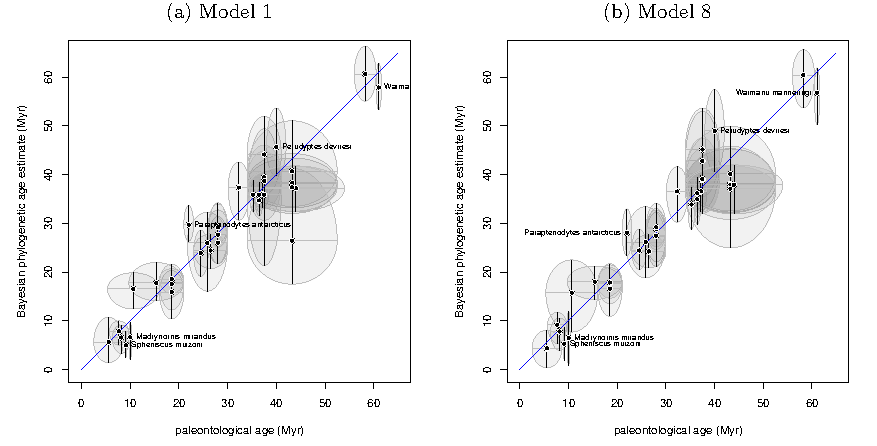
\includegraphics{Figure1.pdf}
\caption{\label{fig:phyloAgeVsGeoAge}
The Bayesian phylogenetic age estimate (median of marginal posterior) for each of the 36 penguin fossils plotted against their palaeontological age estimates, under two alternative site and molecular clock models. The palaeontological age estimates are represented by the mid-point of the range and the upper and lower limits. The Bayesian estimates are represented by the median of the marginal posterior distribution and the upper and lower limits of the 95\% HPD interval. Blue line shows the $x=y$. If the vertical line doesn't cross $x=y$, then the midpoint of the geological range is not in the phylogenetic 95\% HPD. If the horizontal line doesn't cross $x=y$, then the median phylogenetic estimate is not contained in the palaeontological age range. The three labelled fossils show significant inconsistency.}
\end{figure}

\begin{figure}
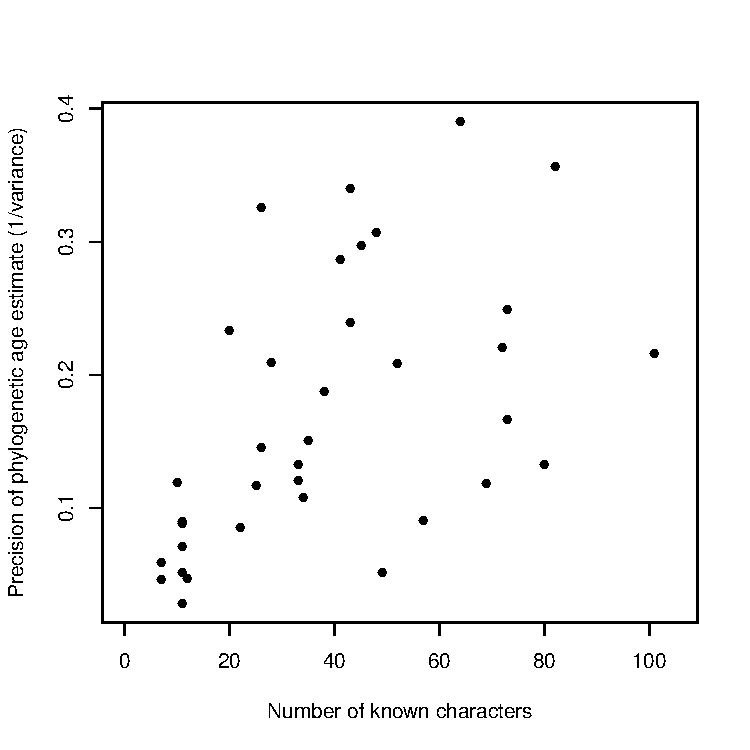
\includegraphics[width=5in]{run8_5/8_precisionVsKnownCharacters.pdf}
\caption{A plot of the number of non-ambiguous morphological sites for the taxon against the precision of the phylogenetic age under \Mrelaxed{} (i.e. the precisions is 1/variance in the marginal posterior distribution of the age).}
\end{figure}

\begin{figure}
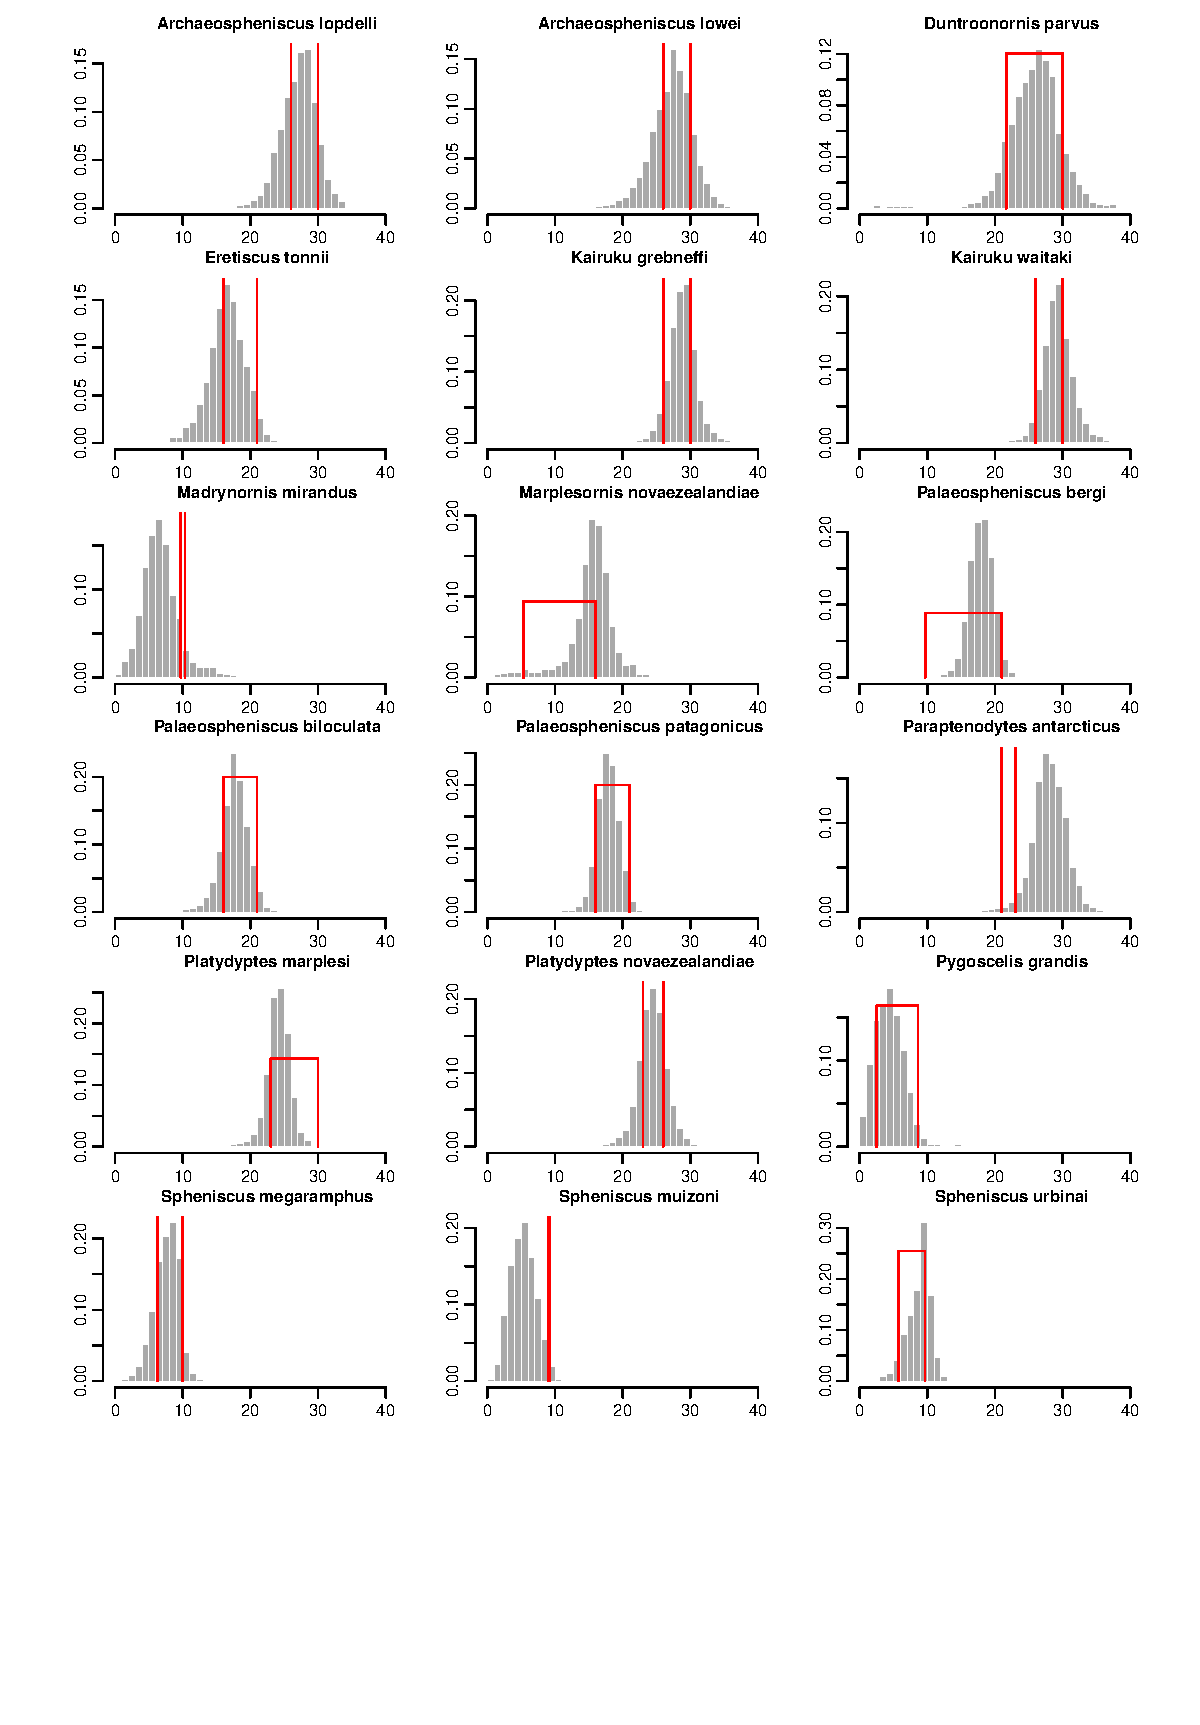
\includegraphics[width=6in]{run8_5/8_fossilDatingHist_younger.pdf}
\caption{\label{hist8_younger}Marginal posterior density plots for the phylogenetic age estimate of each of the 18 penguin fossils younger than 30 Myr using \Mrelaxed{}. Red boxes are the superimposed age ranges derived from geological data.}
\end{figure}

\begin{figure}
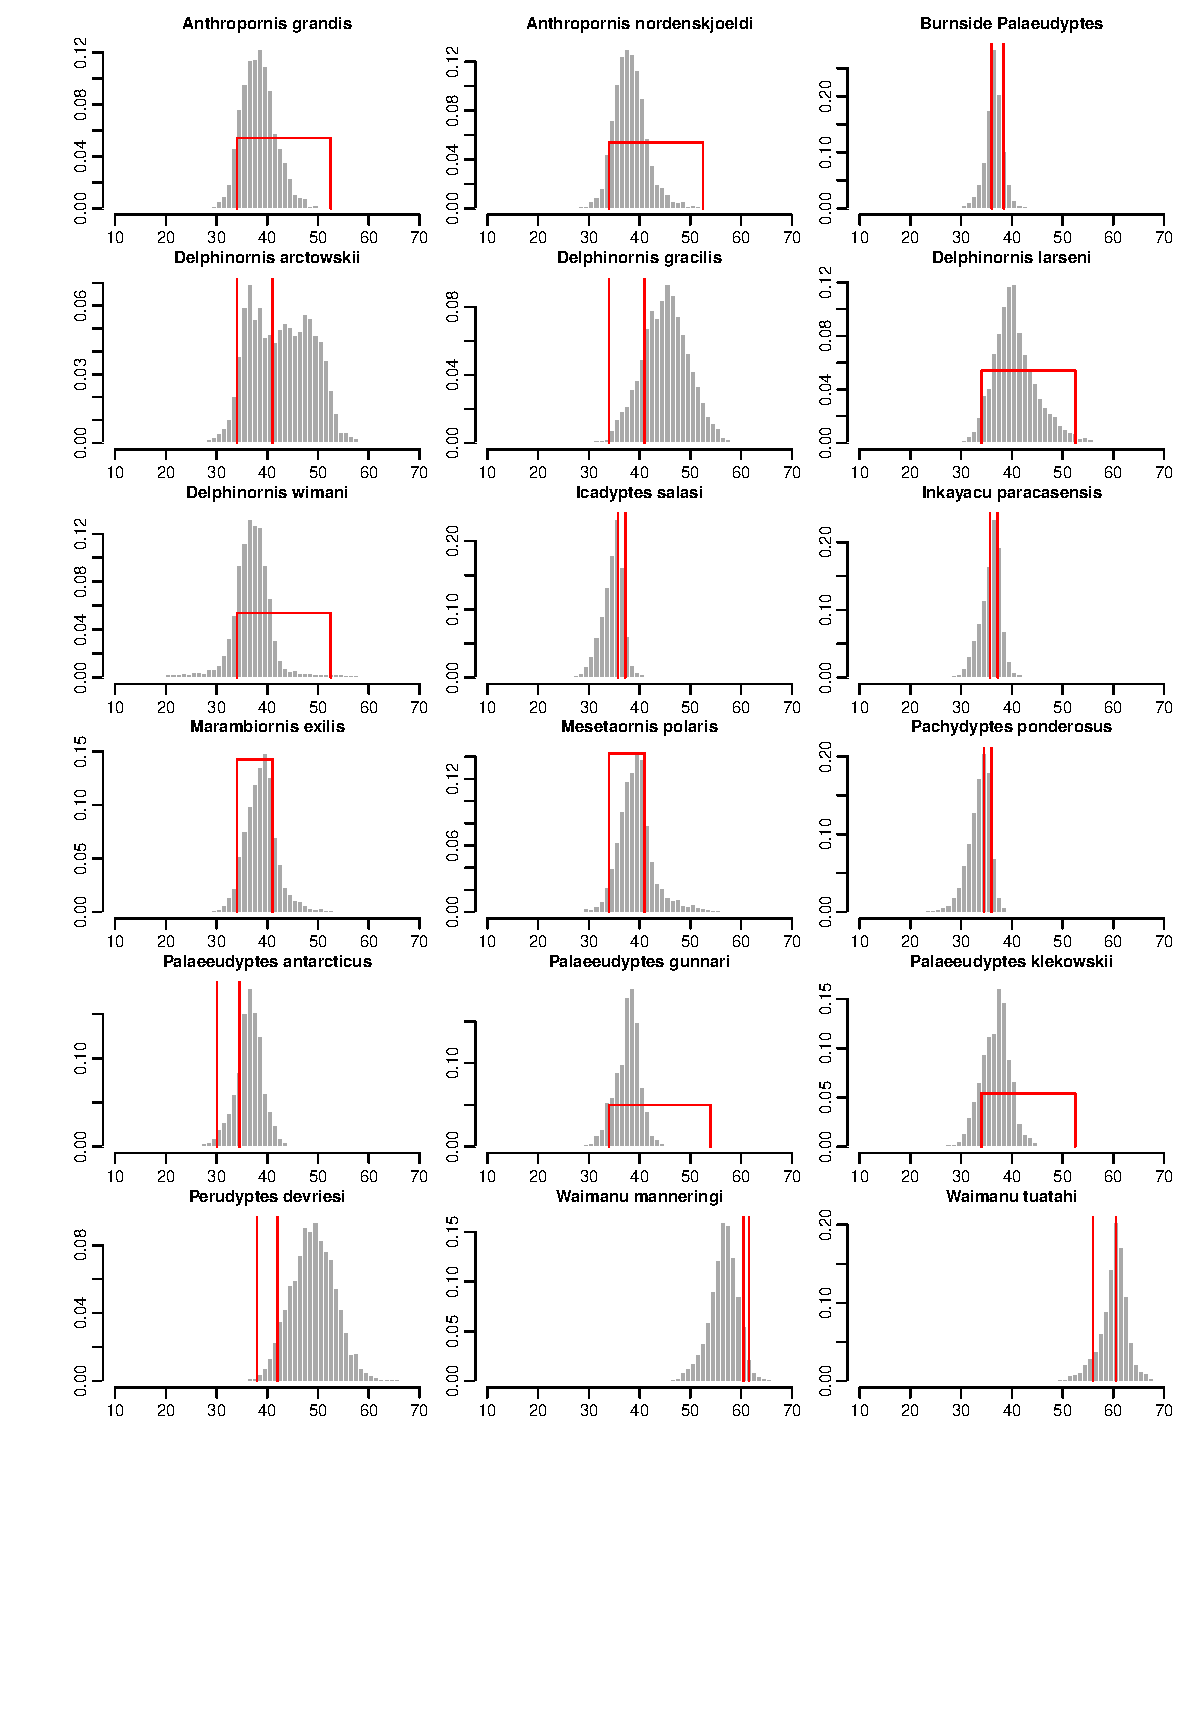
\includegraphics[width=6in]{run8_5/8_fossilDatingHist_older.pdf}
\caption{\label{hist8_older}Marginal posterior density plots for the phylogenetic age estimate of each of the 18 penguin fossils older than 30 Myr using \Mrelaxed{}. Red boxes are the superimposed age ranges derived from geological data.}
\end{figure}

\begin{figure}
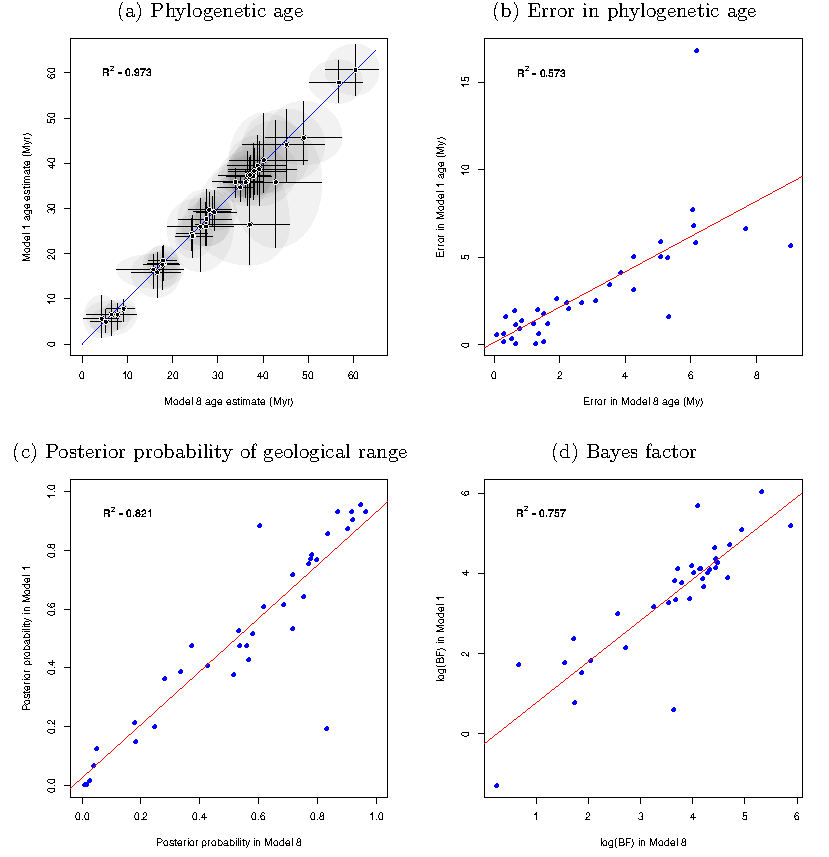
\includegraphics{Figure_comparison.pdf}
\caption{\label{fig:compareM1M8}
Comparison of \Mstrict{} against \Mrelaxed{}. (a) Estimated phylogenetic age of \Mstrict{} against \Mrelaxed{} with $x=y$ line (blue) to guide eye (b) Regression of error in estimated phylogenetic age of \Mstrict{} against \Mrelaxed{}, (c) Regression of posterior probability of palaeontological range of \Mstrict{} against \Mrelaxed{}, (c) Regression of Bayes factor (BF) for palaeontological range of \Mstrict{} against \Mrelaxed{}.}
\end{figure}


% latex table generated in R 3.0.3 by xtable 1.7-4 package
% Sun Aug 16 17:59:05 2015
\begin{table}[ht]
\centering
\begin{tabular}{rrrrrrrr}
  \hline
 & post & BF & phylo age & lower & upper & error & ESS \\ 
  \hline
Anthropornis grandis & 0.94 & 121.8 & 38.4 & 32.8 & 43.9 & 4.9 & 2282 \\ 
  Anthropornis nordenskjoeldi & 0.89 & 61.3 & 37.9 & 31.2 & 44.1 & 5.3 & 2511 \\ 
  Archaeospheniscus lopdelli & 0.50 & 38.5 & 26.4 & 21.5 & 31.3 & 1.6 & 1516 \\ 
  Archaeospheniscus lowei & 0.52 & 41.5 & 27.6 & 21.4 & 33.7 & 0.4 & 2209 \\ 
  Burnside Palaeudyptes & 0.55 & 78.9 & 36.6 & 32.9 & 39.6 & 0.6 & 2132 \\ 
  Delphinornis arctowskii & 0.49 & 20.9 & 36.9 & 20.9 & 48.8 & 0.6 & 369 \\ 
  Delphinornis gracilis & 0.28 & 8.7 & 43.0 & 33.2 & 51.5 & 5.5 & 679 \\ 
  Delphinornis larseni & 0.90 & 70.2 & 39.8 & 31.4 & 50.5 & 3.4 & 761 \\ 
  Delphinornis wimani & 0.20 & 1.9 & 27.0 & 18.4 & 40.9 & 16.3 & 193 \\ 
  Duntroonornis parvus & 0.82 & 82.6 & 25.6 & 18.2 & 30.9 & 0.3 & 2191 \\ 
  Eretiscus tonnii & 0.47 & 27.3 & 15.9 & 10.2 & 20.3 & 2.6 & 3260 \\ 
  Icadyptes salasi & 0.18 & 23.3 & 34.7 & 31.4 & 37.4 & 1.7 & 2824 \\ 
  Inkayacu paracasensis & 0.37 & 62.8 & 35.8 & 32.2 & 38.4 & 0.7 & 3385 \\ 
  Kairuku grebneffi & 0.66 & 76.5 & 29.2 & 25.6 & 32.7 & 1.2 & 4243 \\ 
  Kairuku waitaki & 0.62 & 64.7 & 29.3 & 25.6 & 33.4 & 1.3 & 3987 \\ 
  Madrynornis mirandus & 0.01 & 2.7 & 6.3 & 2.2 & 9.4 & 3.7 & 2722 \\ 
  Marambiornis exilis & 0.68 & 46.8 & 38.9 & 31.8 & 46.5 & 1.4 & 3470 \\ 
  Marplesornis novaezealandiae & 0.37 & 8.1 & 16.6 & 12.4 & 20.1 & 6.0 & 3798 \\ 
  Mesetaornis polaris & 0.68 & 47.3 & 38.9 & 31.9 & 46.7 & 1.4 & 3968 \\ 
  Pachydyptes ponderosus & 0.30 & 44.8 & 36.1 & 32.2 & 38.9 & 0.9 & 2913 \\ 
  Palaeeudyptes antarcticus & 0.16 & 6.7 & 37.0 & 29.9 & 42.4 & 4.7 & 1453 \\ 
  Palaeeudyptes gunnari & 0.88 & 49.6 & 37.3 & 32.0 & 41.7 & 6.7 & 762 \\ 
  Palaeeudyptes klekowskii & 0.86 & 45.3 & 37.3 & 31.7 & 41.9 & 5.9 & 647 \\ 
  Palaeospheniscus bergi & 0.93 & 163.0 & 18.2 & 14.0 & 22.1 & 2.8 & 1249 \\ 
  Palaeospheniscus biloculata & 0.73 & 82.8 & 17.6 & 13.3 & 21.6 & 0.9 & 1111 \\ 
  Palaeospheniscus patagonicus & 0.91 & 328.2 & 18.4 & 15.5 & 21.3 & 0.1 & 1481 \\ 
  Paraptenodytes antarcticus & 0.00 & 0.1 & 29.9 & 26.0 & 33.3 & 7.9 & 2246 \\ 
  Perudyptes devriesi & 0.12 & 5.1 & 45.7 & 38.9 & 53.0 & 5.7 & 1347 \\ 
  Platydyptes marplesi & 0.78 & 77.1 & 24.3 & 20.6 & 27.7 & 2.2 & 4727 \\ 
  Platydyptes novaezealandiae & 0.49 & 50.0 & 23.6 & 18.3 & 28.2 & 0.9 & 5820 \\ 
  Pygoscelis grandis & 0.80 & 101.1 & 5.4 & 1.2 & 10.0 & 0.1 & 2175 \\ 
  Spheniscus megaramphus & 0.58 & 58.9 & 6.7 & 3.3 & 9.6 & 1.5 & 1388 \\ 
  Spheniscus muizoni & 0.00 & 0.6 & 5.1 & 2.5 & 7.8 & 4.0 & 5414 \\ 
  Spheniscus urbinai & 0.83 & 198.0 & 7.8 & 4.8 & 10.3 & 0.2 & 491 \\ 
  Waimanu manneringi & 0.07 & 10.7 & 57.8 & 52.0 & 63.3 & 3.2 & 4239 \\ 
  Waimanu tuatahi & 0.41 & 24.0 & 60.7 & 54.7 & 66.1 & 2.4 & 3898 \\ 
   \hline
\end{tabular}
\caption{Summary of results for 36 fossil penguins under Model 1. {\em post} is the posterior probability that the phylogenetic age is within the paleaontological age range. {\em BF} is the bayes factor in support of the palaeontogical age. {\em phylo age} is the phylogenetic estimate of the age, along with the upper and lower of the corresponding 95\% HPD credible interval. {\em error} is the difference in millions of years between the phylogenetic point estimate of the fossil's age and the mean of it's paleaontological age range. {\em ESS} is the estimated effective sample size for the phylogenetic age estimate.} 
\label{fossilTable1}
\end{table}


% latex table generated in R 3.0.3 by xtable 1.7-4 package
% Mon Aug 17 19:14:22 2015
\begin{table}[ht]
\centering
\begin{tabular}{rrrrrrrr}
  \hline
 & post & BF & phylo age & lower & upper & error & ESS \\ 
  \hline
Anthropornis grandis & 0.92 & 83.0 & 38.2 & 32.3 & 45.3 & 5.1 & 288 \\ 
  Anthropornis nordenskjoeldi & 0.92 & 88.4 & 38.0 & 32.2 & 45.3 & 5.3 & 317 \\ 
  Archaeospheniscus lopdelli & 0.57 & 51.0 & 27.4 & 22.1 & 32.3 & 0.6 & 607 \\ 
  Archaeospheniscus lowei & 0.53 & 44.3 & 27.5 & 21.2 & 33.1 & 0.5 & 616 \\ 
  Burnside Palaeudyptes & 0.54 & 76.2 & 36.6 & 32.3 & 40.0 & 0.6 & 448 \\ 
  Delphinornis arctowskii & 0.37 & 13.0 & 42.8 & 32.8 & 53.0 & 5.3 & 142 \\ 
  Delphinornis gracilis & 0.18 & 4.7 & 45.2 & 35.5 & 53.6 & 7.7 & 401 \\ 
  Delphinornis larseni & 0.95 & 139.7 & 40.2 & 32.5 & 49.9 & 3.1 & 361 \\ 
  Delphinornis wimani & 0.83 & 37.9 & 37.1 & 25.0 & 45.8 & 6.2 & 719 \\ 
  Duntroonornis parvus & 0.78 & 63.4 & 26.1 & 18.8 & 33.4 & 0.3 & 273 \\ 
  Eretiscus tonnii & 0.56 & 39.2 & 16.6 & 10.9 & 21.7 & 1.9 & 873 \\ 
  Icadyptes salasi & 0.25 & 34.6 & 34.9 & 29.8 & 38.2 & 1.5 & 556 \\ 
  Inkayacu paracasensis & 0.34 & 53.5 & 36.2 & 31.1 & 39.4 & 0.3 & 857 \\ 
  Kairuku grebneffi & 0.68 & 84.5 & 28.8 & 24.6 & 32.7 & 0.8 & 950 \\ 
  Kairuku waitaki & 0.62 & 62.5 & 29.2 & 25.2 & 34.1 & 1.2 & 976 \\ 
  Madrynornis mirandus & 0.02 & 6.5 & 6.5 & 0.9 & 12.0 & 3.5 & 432 \\ 
  Marambiornis exilis & 0.75 & 67.0 & 38.8 & 32.0 & 45.3 & 1.3 & 447 \\ 
  Marplesornis novaezealandiae & 0.52 & 15.0 & 15.7 & 7.7 & 22.5 & 5.1 & 468 \\ 
  Mesetaornis polaris & 0.72 & 55.6 & 39.1 & 32.4 & 47.5 & 1.6 & 470 \\ 
  Pachydyptes ponderosus & 0.28 & 41.0 & 33.9 & 28.7 & 37.4 & 1.4 & 1478 \\ 
  Palaeeudyptes antarcticus & 0.18 & 7.8 & 36.6 & 30.2 & 41.6 & 4.3 & 400 \\ 
  Palaeeudyptes gunnari & 0.90 & 66.4 & 37.9 & 31.9 & 42.0 & 6.1 & 274 \\ 
  Palaeeudyptes klekowskii & 0.84 & 38.8 & 37.1 & 30.8 & 41.8 & 6.1 & 248 \\ 
  Palaeospheniscus bergi & 0.96 & 354.5 & 18.0 & 14.4 & 21.2 & 2.7 & 378 \\ 
  Palaeospheniscus biloculata & 0.78 & 111.2 & 17.7 & 13.5 & 21.4 & 0.8 & 421 \\ 
  Palaeospheniscus patagonicus & 0.87 & 205.1 & 17.9 & 14.6 & 20.9 & 0.6 & 306 \\ 
  Paraptenodytes antarcticus & 0.02 & 1.3 & 28.1 & 23.4 & 33.0 & 6.1 & 752 \\ 
  Perudyptes devriesi & 0.05 & 1.9 & 49.0 & 40.6 & 57.5 & 9.0 & 735 \\ 
  Platydyptes marplesi & 0.80 & 85.7 & 24.2 & 20.9 & 27.7 & 2.3 & 795 \\ 
  Platydyptes novaezealandiae & 0.58 & 72.6 & 24.4 & 20.5 & 28.8 & 0.1 & 527 \\ 
  Pygoscelis grandis & 0.77 & 85.1 & 4.3 & 0.3 & 8.0 & 1.3 & 697 \\ 
  Spheniscus megaramphus & 0.72 & 107.1 & 7.8 & 3.9 & 10.5 & 0.4 & 473 \\ 
  Spheniscus muizoni & 0.01 & 5.7 & 5.3 & 1.9 & 8.7 & 3.8 & 1466 \\ 
  Spheniscus urbinai & 0.60 & 60.4 & 9.2 & 5.3 & 11.7 & 1.5 & 276 \\ 
  Waimanu manneringi & 0.04 & 5.6 & 56.8 & 50.2 & 61.9 & 4.3 & 1010 \\ 
  Waimanu tuatahi & 0.43 & 25.7 & 60.5 & 53.7 & 65.6 & 2.2 & 918 \\ 
   \hline
\end{tabular}
\caption{Summary of results for 36 fossil penguins under Model 8. {\em post} is the posterior probability that the phylogenetic age is within the paleaontological age range. {\em BF} is the bayes factor in support of the palaeontogical age. {\em phylo age} is the phylogenetic estimate of the age, along with the upper and lower of the corresponding 95\% HPD credible interval. {\em error} is the difference in millions of years between the phylogenetic point estimate of the fossil's age and the mean of it's paleaontological age range. {\em ESS} is the estimated effective sample size for the phylogenetic age estimate.} 
\label{fossilTable8}
\end{table}


\section*{Discussion}

In this paper we have demonstrated that even a small number of morphological characters (some of the fossils had as few as 7 morphological traits coded) can be used in the context of a rich fossil reference data set, to provide an accurate and precise age of the fossil based on a phylogenetic model. 
There are a diverse array of potential applications for this methodology. 
The most obvious is the estimation of dates for fossils that are temporally unconstrained, either due to poor knowledge of the age of the sediments in which it was found or a complete lack of provenance data (e.g. a recent fossil described as a `four-legged snake' has excited controversy for a lack of provenance\footnote{See \url{http://news.sciencemag.org/paleontology/2015/07/four-legged-snake-fossil-stuns-scientists-and-ignites-controversy}}). 
It can also be used a way of testing the ``morphological clock'' and to discover potential problems in the data by identifying outlier fossils with respect to model fit. 
The median error in age estimates for the penguin data set we analysed here was 2 My, using either a very simple or a more complex model of discrete morphological change. In both cases we used the new fossilized birth-death tree prior, which is a crucial ingredient in allowing for the estimating of fossil ages under a birth-death tree prior.

\printbibliography


\end{document}
